\documentclass[12pt,a4paper]{report}
\usepackage{graphicx}
\usepackage{pdfpages}
\usepackage{hyperref}
\usepackage{wrapfig}
\usepackage{lscape}
\usepackage{rotating}
\usepackage{epstopdf}
\usepackage[utf8]{inputenc}
\usepackage[cyr]{aeguill}
\usepackage[francais]{babel}\usepackage{listings}
\usepackage{xcolor}
\usepackage{textcomp}
\lstset{literate=
{\'{e}}{{\'e}}1
{à}{{\`a}}1
{â}{{\^a}}1
}
\definecolor{orange}{rgb}{0.8,0.4,0.0}
\definecolor{darkblue}{rgb}{0.0,0.0,0.6}
\definecolor{cyan}{rgb}{0.0,0.6,0.6}
\lstdefinelanguage{JSON}
{
   basicstyle=\normalsize,
   columns=fullflexible,
   showstringspaces=false,
   commentstyle=\color{gray}\upshape,
   morestring=[b]",
   morestring=[s]{>}{<},
   morecomment=[s]{<?}{?>},
   stringstyle=\color{orange},
   identifierstyle=\color{darkblue},
   keywordstyle=\color{blue},
   morekeywords={string,number,array,object}% list your attributes here
}
\graphicspath{ {images/} }
\hypersetup{
    colorlinks,
    citecolor=black,
    filecolor=black,
    linkcolor=black,
    urlcolor=black
}
\begin{document}
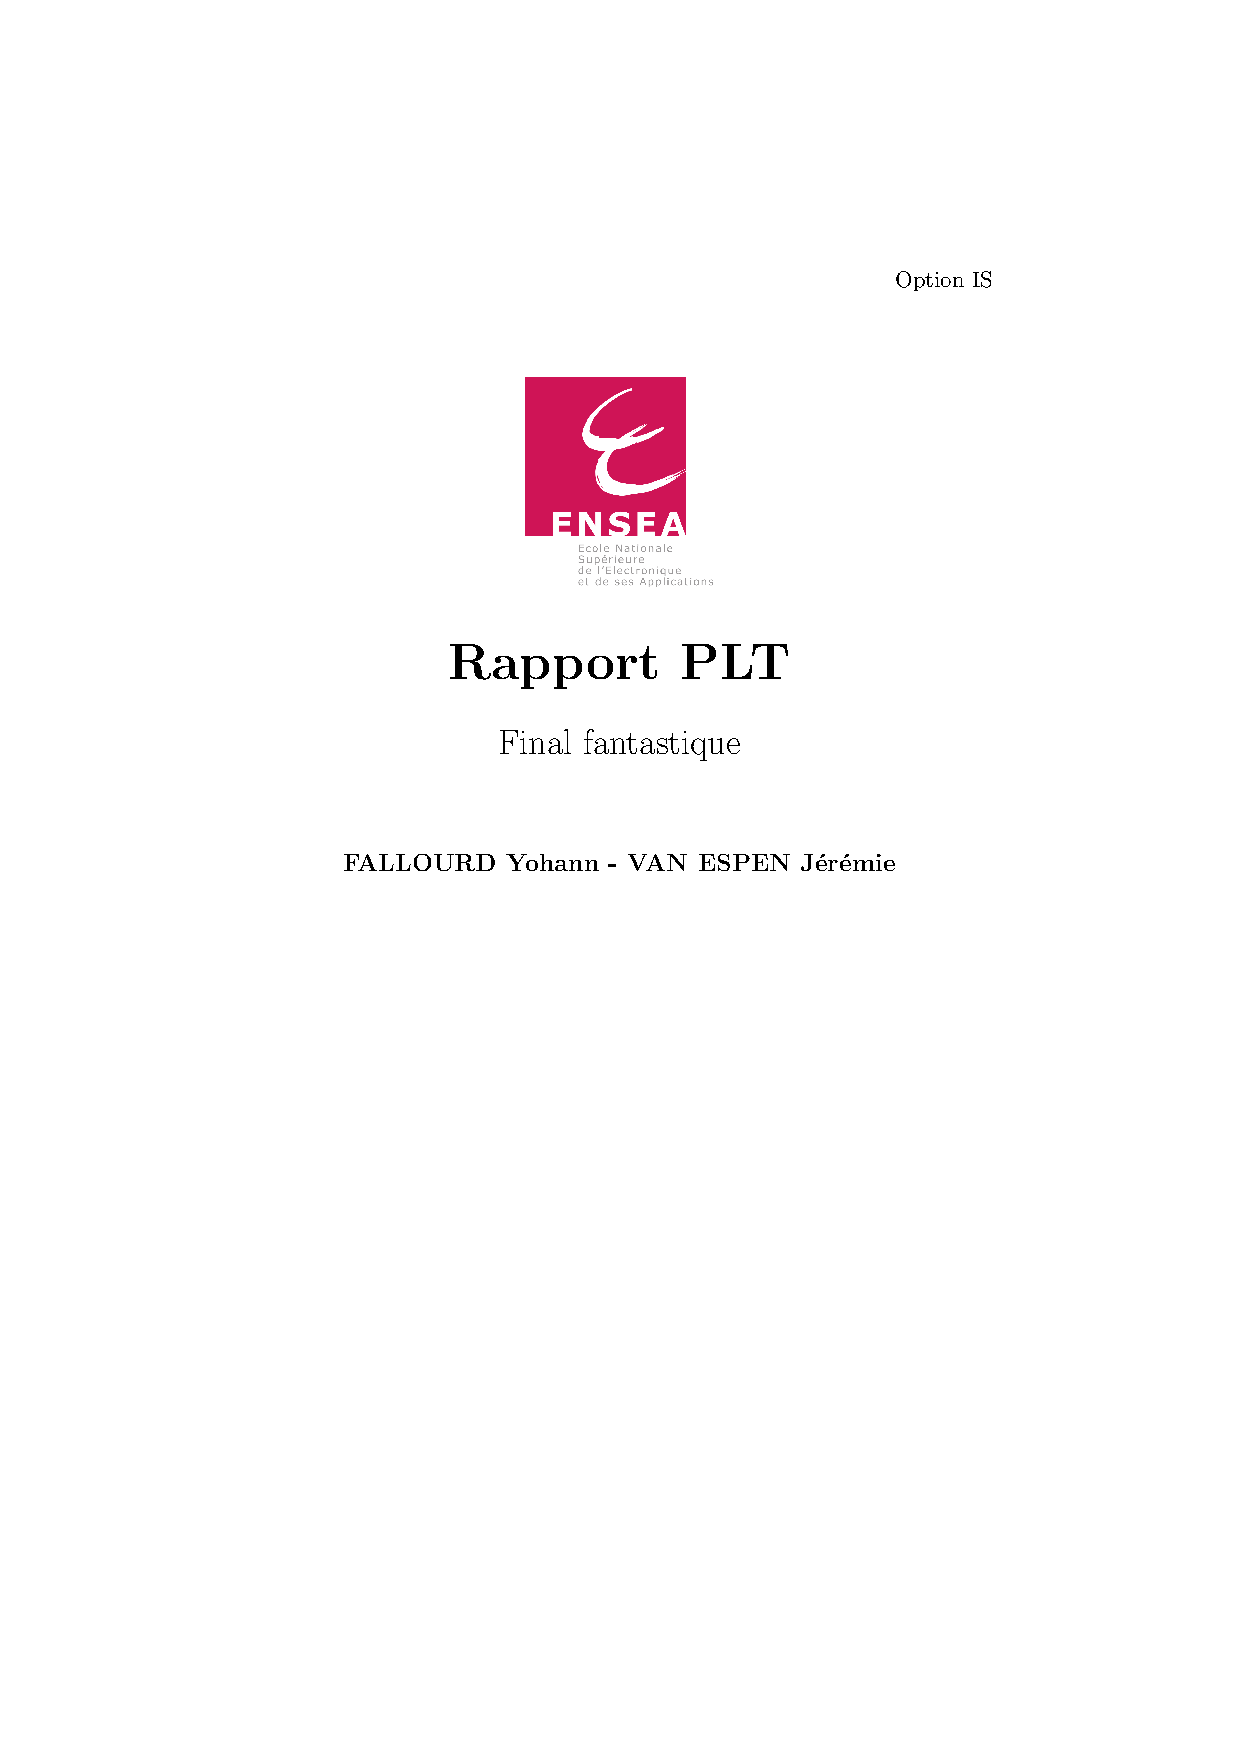
\includepdf{Titlepage}
\tableofcontents
\chapter{Objectif}
\section{Pr\'{e}sentation g\'{e}n\'{e}rale}
Le jeu est bas\'{e} sur l'arch\'{e}type de Final Fantasy X, se distinguant par un syst\`{e}me de combat au tour par tour ainsi que son embl\'{e}matique "sph\'{e}rier" correspondant à un arbre de talent apportant une libert\'{e} de personnalisation non n\'{e}gligeable. Voici un croquis du sph\'{e}rier :

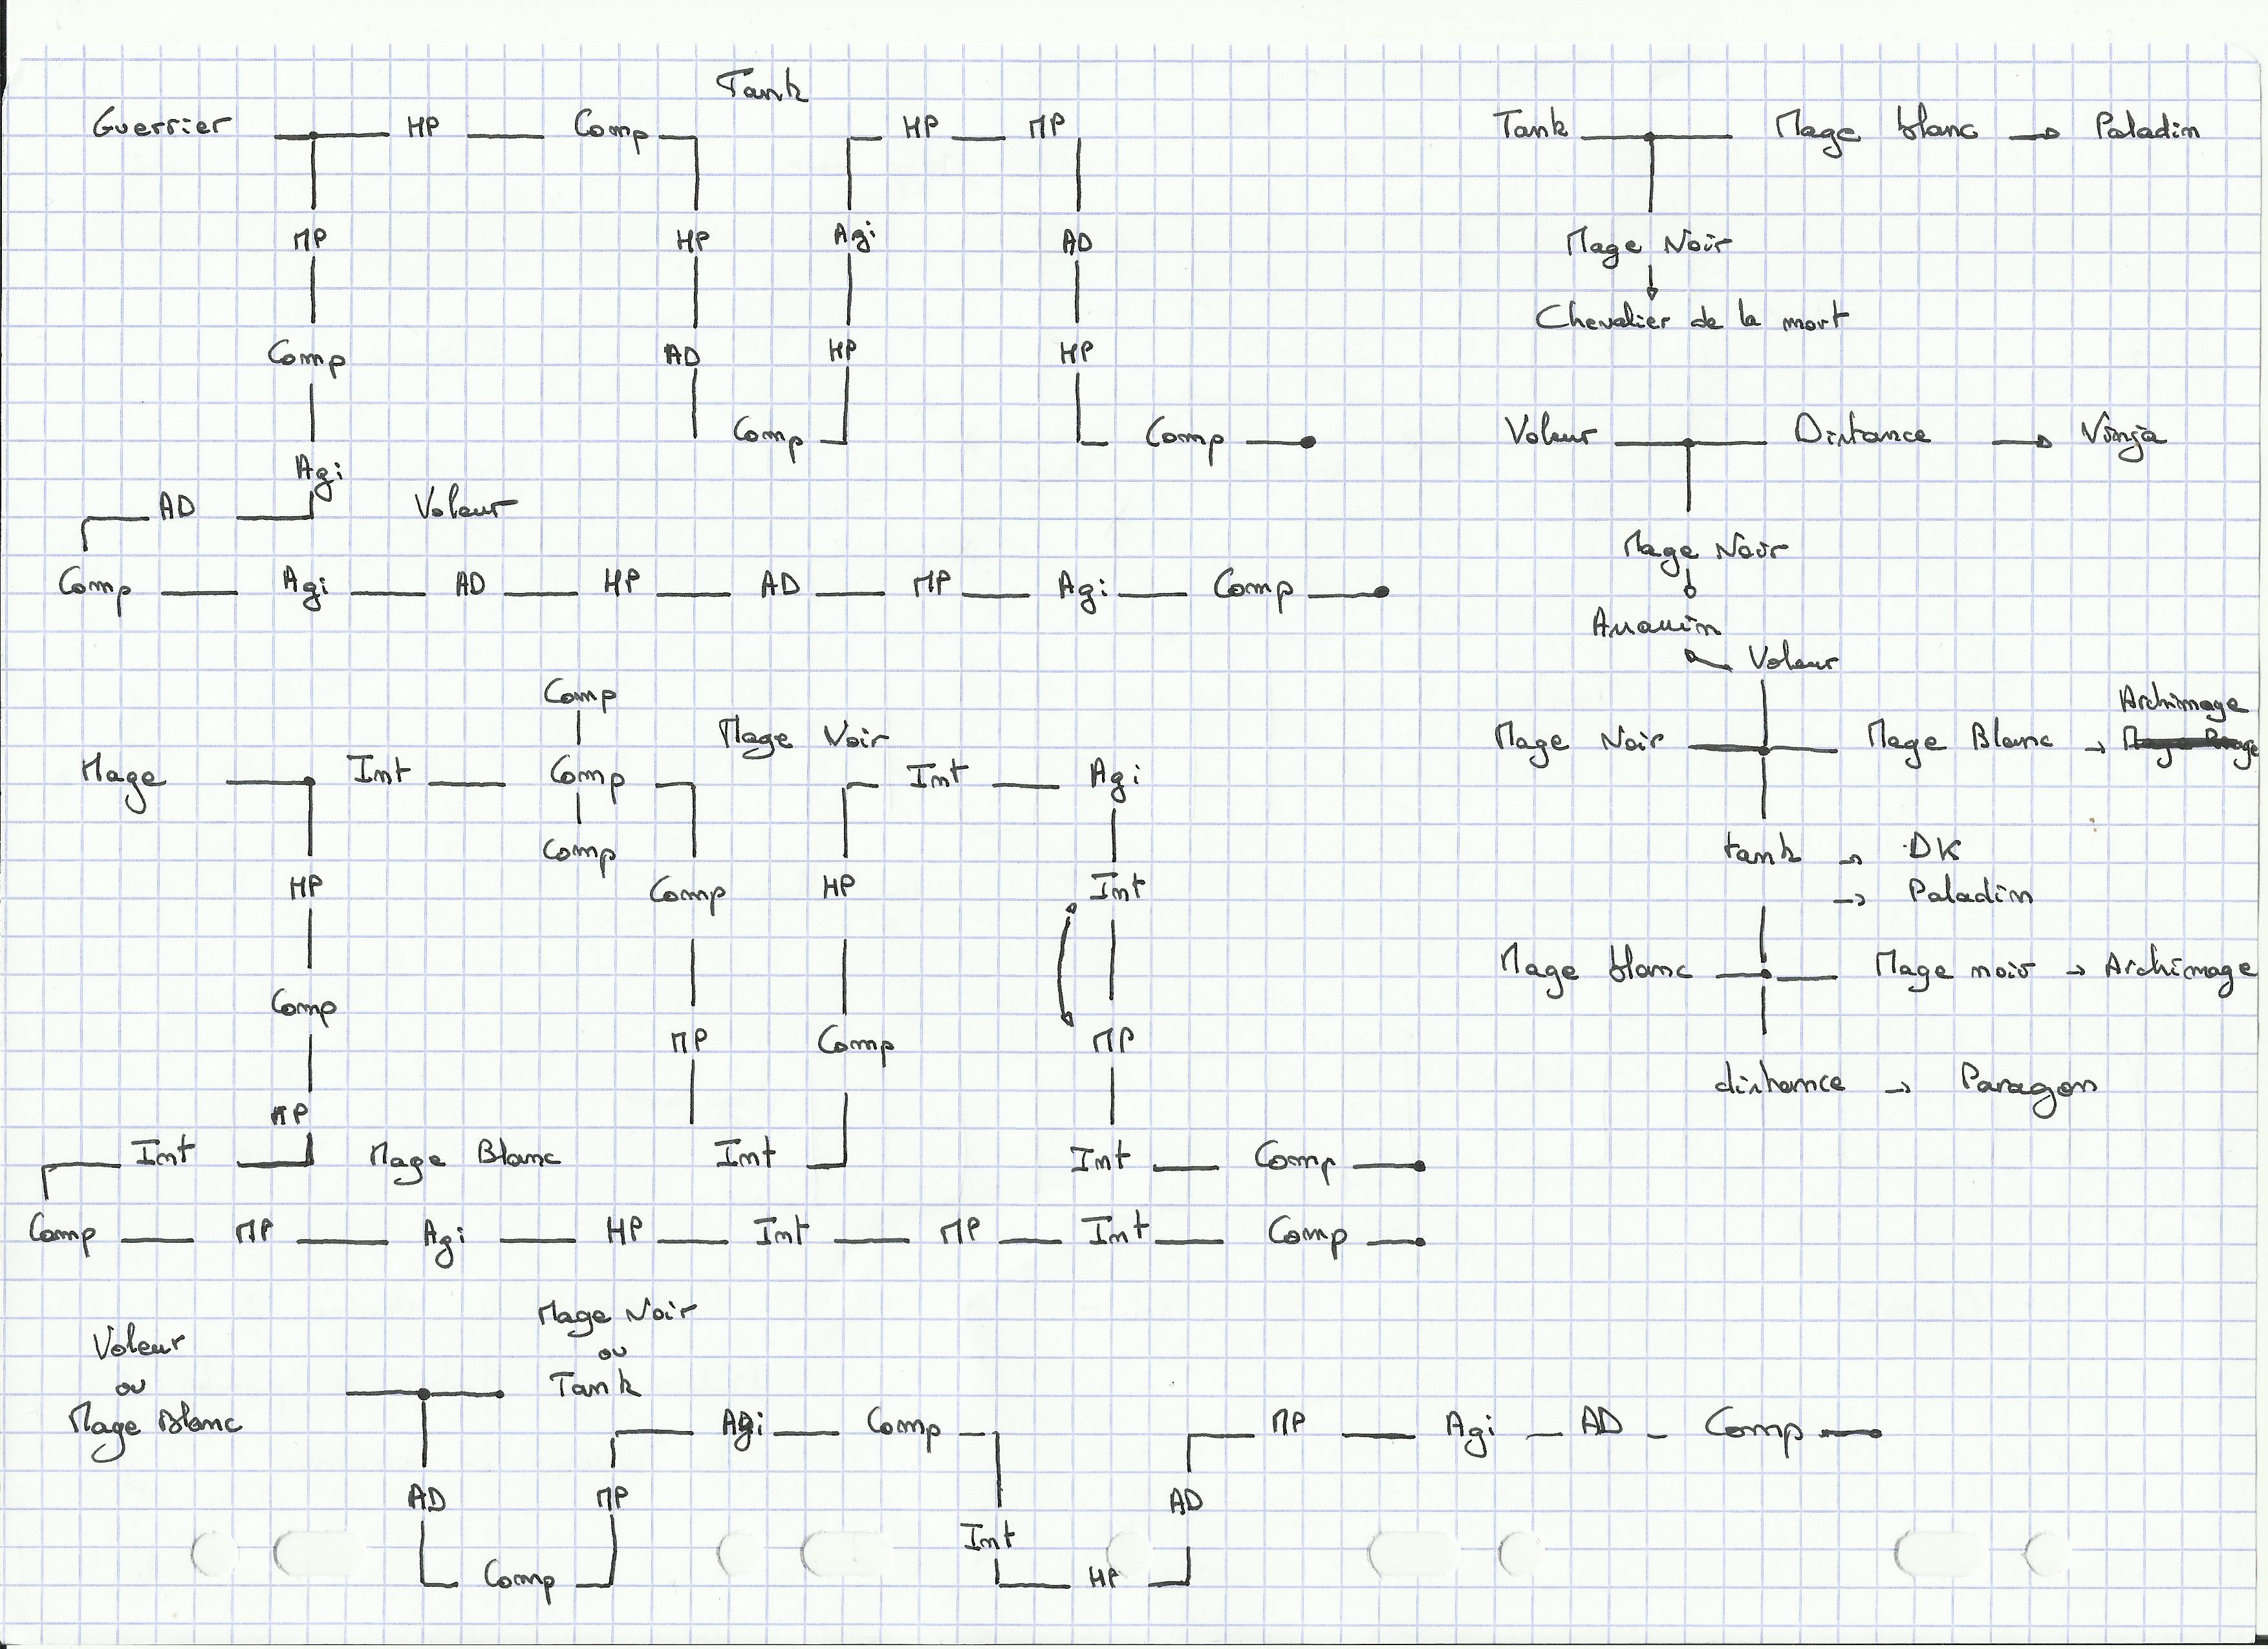
\includegraphics[width=0.80\textwidth]{Spherier.jpg}

A la diff\'{e}rence du v\'{e}ritable jeu, il n'y aura pas de d\'{e}placement libre en temps r\'{e}el; le gameplay se r\'{e}sume à un d\'{e}placement de points d'int\'{e}rêts en points d'int\'{e}rêts, pouss\'{e} par une histoire typique de cet arch\'{e}type, où se d\'{e}roulent diff\'{e}rents \'{e}v\`{e}nements/combats.



\section{R\`{e}gles du jeu}
Le coeur du jeu sont les deux personnages auquel le joueur (si il joue seul) a acc\`{e}s. Chacun commence avec une sp\'{e}cialisation particuli\`{e}re de mage et de guerrier choisissant directement de se diriger vers diff\'{e}rentes sp\'{e}cialisations. Via une carte du monde, le joueur avance de point en point et d\'{e}clenche diff\'{e}rentes rencontres. Les combats se d\'{e}roulent en tour par tour et si l'un des joueurs meurt, il revient à la vie avec 1 point de vie. La mort des deux joueurs entraine un retour au dernier point de sauvegarde automatique. Gagner un combat donne de l'exp\'{e}rience, qui donne des niveaux, qui permettent de progresser dans le sph\'{e}rier. 

Il existe \'{e}galement diff\'{e}rents objets permettant de rendre de la vie ou d'avoir d'autres effets. De plus, un syst\`{e}me d'\'{e}quipement existe pour rendre le joueur plus fort au cours de l'aventure. En effet, un personnage poss\`{e}de des caract\'{e}ristiques (Force, Agilit\'{e}, Intelligence, Points de vie (HP) et Points de magie (MP)) qu'il peut am\'{e}liorer.

Le jeu se finit lorsque l'aventure est termin\'{e}e !
\section{Conception Logiciel}

Voici les packages de notre projet :

\textbf{Package state.} Package central qui g\`{e}re l'\'{e}tat du jeu.

\textbf{Package engine.} Package qui modifie l'\'{e}tat de jeu et stocke les commandes.

\textbf{Package ai.} Package qui g\`{e}re le contrôle par l'ordinateur des monstres et, potentiellement, un personnage principal.

\textbf{Package server.} Package contenant la gestion de l'API du jeu, que ce soit par r\'{e}seau ou localement.

\textbf{Package instance.} Package contenant l'Interface Homme-Machine.

\textbf{Package render.} Package contenant la gestion du rendu.

\begin{figure}
\caption{Diagramme des packages}
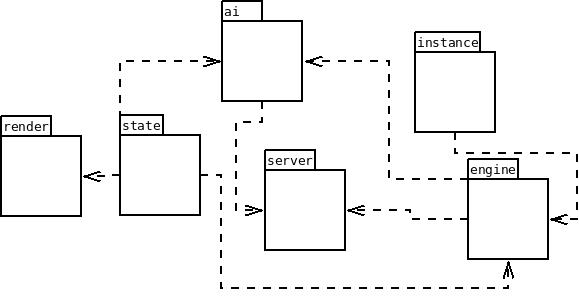
\includegraphics[width=0.80\textwidth]{packdia.jpeg}
\end{figure}

\chapter{Description et conception des \'{e}tats}
\section{Description des \'{e}tats}

Un \'{e}tat du jeu est form\'{e} par un ensemble d'\'{e}l\'{e}ments vivants et non vivants ainsi que la situation dont se trouve le joueur.

\subsection{Etat \'{e}l\'{e}ments vivants}

Les \'{e}l\'{e}ments vivants sont des entit\'{e}s ayant tous des caract\'{e}ristiques propres : sant\'{e} max, sant\'{e} actuelle, mana max, mana actuel, force, agilit\'{e} et intelligence.
On distingue deux types d'\'{e}l\'{e}ments vivants :

\textbf{Character.} Ce sont les h\'{e}ros du jeu. Ils pourront s'\'{e}quiper d'une arme et d'une protection ajoutant des bonus d'attaque et de d\'{e}fence. Ils \'{e}volueront grâce \`{a} un syst\`{e}me de gain d'exp\'{e}rience et de personalisation du joueur.  

\textbf{Monster.} Comme le nom l'indique, ce sont les monstres du jeu. Ils ne peuvent pas gagner d'exp\'{e}rience et leurs caract\'{e}ristiques sont g\'{e}n\'{e}r\'{e}es avec le niveau actuel des h\'{e}ros. Leurs comp\'{e}tences seront fix\'{e}es suivant le type du monstre (\'{e}l\'{e}mentaire, boss ect...). Ils ne portent pas d'\'{e}quipement. Seul les boss auront une capacit\'{e} sp\'{e}ciale (comme les h\'{e}ros) appel\'{e} "Overdrive".

\subsection{Etat \'{e}l\'{e}ments non vivants}

Les \'{e}l\'{e}ments non vivants sont au nombre de trois et ne portent aucune caract\'{e}ristiques communes. 

\textbf{Item.} Ce sont les objets utilisables par les h\'{e}ros. Ils peuvent changer leurs attributs (augmentation d'une caract\'{e}ristique ect...).

\textbf{SphereGrid.} C'est une table des comp\'{e}tences. Chaque niveaux suppl\'{e}mentaires permettra au character d'apprendre de nouvelles comp\'{e}tences et d'augmenter ces caract\'{e}ristiques. Il sera possible au joueur de choisir la personnalisation de son personnage car plusieurs table sont possible au cours du jeu.   

\textbf{Node.} Ce sont les points clefs du jeu. Les h\'{e}ros pourront se d\'{e}placer sur une carte de noeud en noeud. Chaque noeud comporte des \'{e}v\`{e}nements al\'{e}atoires et non al\'{e}atoires. Les \'{e}l\'{e}ments al\'{e}atoires sont des combats contre des monstres al\'{e}atoires tandis que les non al\'{e}atoires sont des \'{e}l\`{e}ments de l'histoire. Cela peut \^{e}tre un simple dialogue ou un combat contre un boss. Il est possible uniquement de ce d\'{e}placer au noeud suivant ou au noeud pr\'{e}c\'{e}dent. Si ce noeud a d\'{e}j\`{a} \'{e}t\'{e} visit\'{e}, l'\'{e}v\`{e}nement non al\'{e}atoire n'aura plus lieu.

\subsection{Situation du joueur}

Les situations possibles dans lequelles se trouve le joueur sont au nombre de quatre. Elles repr\'{e}sentent la ligne directive du jeu.

\textbf{D\'{e}placement sur un noeud.} Le joueur se d\'{e}place dans un nouvel endroit qui va g\'{e}n\'{e}rer des \'{e}v\`{e}nements. 

\textbf{Ev\`{e}nement al\'{e}atoire.} Cet \'{e}v\`{e}nement se traduit la plus part du temps par un combat contre des monstres al\'{e}atoires.

\textbf{Aubergiste.} En arrivant dans un nouveau lieu, le joueur a acc\`{e}s \`{a} un menu lui permettant d'acheter des objets utilisables en combat et de se pr\'{e}parer \`{a} l'\'{e}v\`{e}nement non al\'{e}atoire.

\textbf{Ev\'{e}nement non al\'{e}atoire.} Il d\'{e}pend de l'histoire du jeu.

\newpage

\section{Conception logiciel}

Dans cette section, nous expliciterons le diagrammes des classes pour les \'{e}tats pr\'{e}sent\'{e} en fin de chapitre. 

\textbf{Classes Element.} Cette classe et ses classes filles contiennent tout les \'{e}l\'{e}ments vivants du jeu. On distingue deux classes filles : Character et Monster. La classe Character poss\`{e}de des d\'{e}pendances avec des classes comme SphereGrid et Item qui repr\'{e}sentent l'\'{e}volution des personnages ainsi que les objets dont ils pourront faire l'usage. 

\textbf{Liste d'\'{e}l\'{e}ments.} Elle va contenir toute les informations sur l'ensemble des \'{e}l\'{e}ments pr\'{e}sent dans le jeu. 

\textbf{Classes Node.} Cette classe permet de faire le lien entre l'apparition d'\'{e}v\`{e}nements et les \'{e}l\'{e}ments. C'est une liste chain\'{e}e dont le d\'{e}placement est bidirectionnel. 

\textbf{Classe State.} Cette classe contiendra toutes les informations li\'{e}es au noeud o\`{u} se trouve le joueur et aux \'{e}l\'{e}ments vivants / non vivants encore pr\'{e}sent.

\textbf{Observer.} Cette classe permettra de relever les changements d'\'{e}tats du jeu et de le transmettre aux autres packages.


\chapter{Rendu : Strat\'{e}gie et Conception}
\section{Strat\'{e}gie de rendu d'un \'{e}tat}
Notre jeu \'{e}tant à temps discret, le rendu d'un \'{e}tat sera assez simple. Le tout \'{e}tant de distinguer entre le rendu et l'IHM qui correspond au menu.

Pour se faire, nous introduisons le concept d'instance, offrant une classe par contexte (ie. Combat, Carte du monde, Menu d'intro...) g\'{e}rant l'IHM pour chaque environnement. Le rendu sera fait par les classes du package render en associant un Renderer à chaque contexte.

\section{Conception logiciel}

\textbf{Renderer.} Cette classe contient toutes les informations communes entre chaque contexte. Elle est n\'{e}anmoins abstraite et ses classes filles (WorldMapRender, FightRender ...) doivent ainsi red\'{e}finir ces m\'{e}thodes afin de diff\'{e}rencier correctement chaque contexte et chaque \'{e}tat du jeu.

\textbf{TextureSetter.} C'est dans cette classe que l'on va instancier toutes les textures des \'{e}l\'{e}ments vivants et non vivants du jeu. Ce tableau sera utilis\'{e} par les classes filles de Renderer.


\chapter{R\`{e}gle de changement d'\'{e}tat}

Le jeu est \`{a} temps discret donc les changements d'\'{e}tats ne se feront uniquement lors d'appuis sur des touches du clavier par l'utilisateur. Chaque contexte offre des choix diff\'{e}rents \`{a} l'utilisateur. 

\section{Conception logiciel}

\textbf{Screen.} C'est la classe m\`{e}re du package. Elle fait le lien entre la classe Application, ses classes filles et le package state afin de lier l'\'{e}tat et le rendu.

\textbf{Application.} Cette classe fait le lien entre la biblioth\`{e}que SFML et les diff\'{e}rents \'{e}tats du jeu. En effet \`{a} chaque nouvel \'{e}tat nous aurons \`{a} instancier de nouveaux sprites.

\textbf{Info, Worldmap, Fight, Inn.} Les classes filles de Screen nous permette de mieux personaliser les contextes suivant les choix de l'utilisateur et sa position dans l'histoire du jeu.


\chapter{IA}

\section{Comportement}

L'intelligence artificielle peut g\'{e}rer les personnages comme les monstres du jeux. Son comportement est dict\'{e} par la classe Rules (pr\'{e}sent dans le package engine) avec les deux variables bool\'{e}ennes AICharneeded et AIMonsterneeded.
Dans notre cas, l'intelligence artificielle doit choisir une action \`{a} effectuer sur une cible. Une premi\`{e}re i.a. devra choisir al\'{e}atoirement une action ainsi que sa cible, une seconde devra effectuer une action al\'{e}atoirement mais sur la meilleure cible et enfin une troisi\`{e}me devra choisir l'action la plus rentable sur la meilleure des cibles.
Pour cela nous utiliserons deux classes types : AI et ChoiceList.

\textbf{AI.} Cette classe contient toutes les informations dont \`{a} besoin une intelligence artificielle pour fonctionner. Les variables ChoiceTarget et ChoiceAction sont r\'{e}cup\'{e}r\'{e}es par l'engine qui devra actualiser l'\'{e}tat du jeu. Les sous classes RandomChoice et RandomGoodChoice sont les intelligences artificielles premi\`{e}res et secondes cit\'{e}es plus haut. La classe SmartChoice est ainsi la troisi\`{e}me.

\textbf{ChoiceList.} Cette classe permet de cr\'{e}er un tableau avec les divers actions possibles sur n'importe quelles cibles. Ce tableau sera plus moins restreint suivant les besoins de l'intelligence artificielle utilis\'{e}e. Par exemple, l'i.a. RandomChoice aura besoin de toutes les combinaisons possibles d'action et de cible alors que RandomGoodChoice fera un premier tri sur les cibles suivant l'action execut\'{e}e. La restriction du tableau suivant les diff\'{e}rentes cibles possibles pour une action se base sur des param\`{e}tres logiques. Ainsi les actions d\'{e}fensives ne pourront pas \^{e}tre lanc\'{e}es sur des ennemies.

\section{Intelligence artificielle haut niveau}

L'intelligence artificielle dite de haut niveau (intitul\'{e} SmartChoice) s'appuit sur le parcours d'arbre de possibilit\'{e}s. En partant du tableau utilis\'{e} par l'i.a. RandomGoodChoice (qui conserve la meilleure cible pour une action donn\'{e}e), elle applique un algorithme appel\'{e} algorithme de MinMax. Cette algorithme a pour r\^{o}le de retourner une map avec comme clef les diff\'{e}rentes actions possibles et comme valeur li\'{e}e \`{a} cette clef son gain maximum. Le calcul de gain pour chaque action se fait suivant une fonction de pond\'{e}ration pr\'{e}sente dans la classe ChoiceList et le gain maximum est donc la somme du gain d'une action avec le gain le plus grand ou le plus faible de l'action du joueur suivant s'il est un alli\'{e} ou un ennemi. Avec cette map, l'i.a. d\'{e}cide de jouer l'action ayant le gain "max" le plus \'{e}lev\'{e} sur la meilleure cible, selectionn\'{e} pr\'{e}alablement avec le tableau de l'i.a. RandomGoodChoice. 

\begin{sidewaysfigure}[ht]
\caption{Diagramme de classe du package ai}
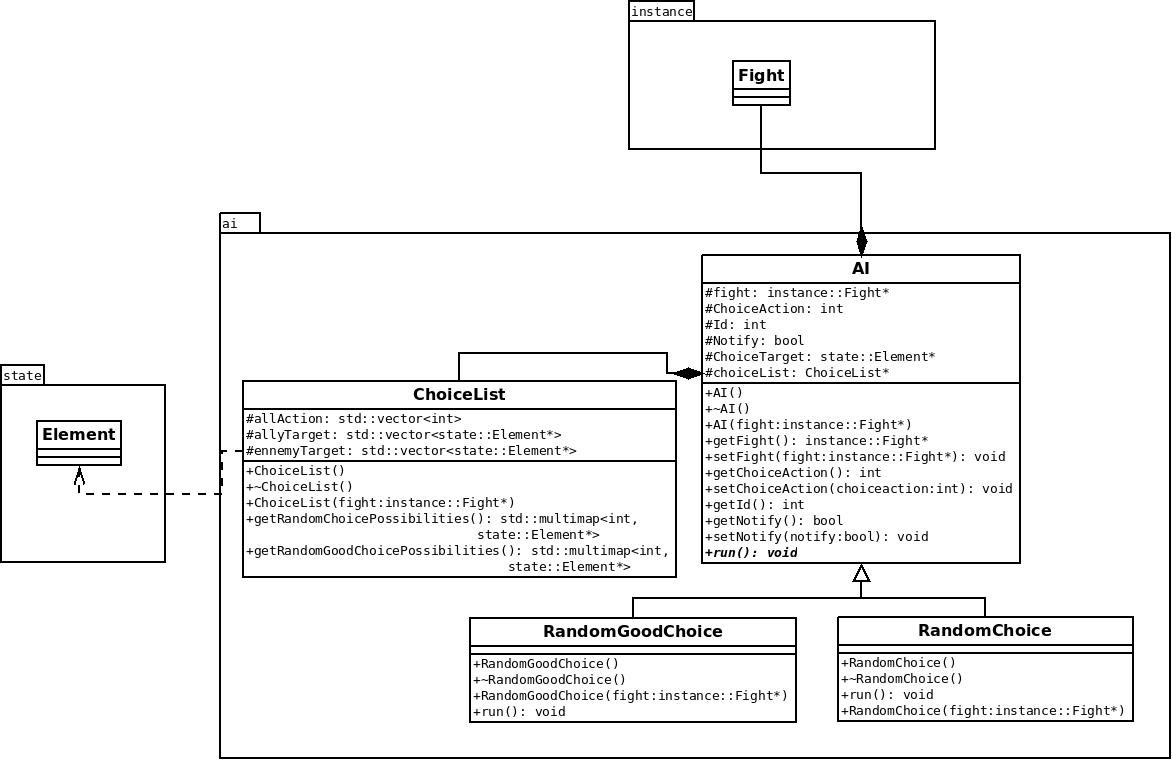
\includegraphics[width=1\textwidth]{ai.jpeg}
\end{sidewaysfigure}

\chapter{Engine et modularisation}

L'engine a pour but de stocker les commandes g\'{e}n\'{e}r\'{e}es par l'utilisateur ou l'IA avant qu'un thread parall\`{e}le au principal vide le tableau de commandes et les ex\'{e}cute.

\section{Stockage de commandes}

Les commandes envoy\'{e}es par l'IHM sont de deux types diff\'{e}rents : MoveInUI correspondant au changement d'\'{e}tat associ\'{e} \'{a} un d\'{e}placement dans le menu et Action correspondant aux diff\'{e}rentes actions lors d'un combat (attaque, objet, soin, etc..). Ces commandes sont stock\'{e}es dans un tableau de l'engine en attendant que le thread secondaire les ex\'{e}cute.

\section{Ex\'{e}cution des commandes}

Le thread secondaire est pris dans une boucle infinie dans laquelle il transf\`{e}re les commandes dans un tableau secondaire avant de le lock et d'ex\'{e}cuter toutes les commandes. Le tableau secondaire permet de ne pas locker le tableau principal, ce qui agirait comme un bottleneck dans l'ajout de commandes par l'IHM.

\chapter{Server : conception de l'API}

\section{API REST}
La partie serveur de l'API est instaurée via la librairie Pistache tandis que la partie client est instaurée via Chilkat.

Le but de l'API est de rassembler les diff\'{e}rentes commandes g\'{e}n\'{e}r\'{e}es sur un serveur distant avant que le client ne les r\'{e}cup\`{e}re pour les ex\'{e}cuter mais aussi d'offrir les services CRUD sur une base de données d'utilisateurs.

\subsection{Envoi des commandes au serveur}

\textbf{Requête :} PUT /cmd

\textbf{Données requête :} 

\begin{lstlisting}[language=JSON]
type: "object",
properties: {
   "unixtime": { type:number },
   "cmdtype": { type:string, pattern: "(action|moveinui)" },
   "action": { type:number, minimum:0, maximum:16 },
   "casterindex": { type:number, minimum:0},
   "targetindex": { type:number, minimum:0},
required: [ "unixtime", "cmdtype", "action", "casterindex", "targetindex" ]
\end{lstlisting}


\textbf{Réponse :} STATUS 200 si OK, STATUS 500 si une erreur est survenue.

\subsection{Récupération des commandes}

\textbf{Requête :} GET /cmd


\textbf{Réponse :} STATUS 200 si OK, STATUS 404 si aucune commande n'est sur le serveur.

\textbf{Données Réponse :} 

\begin{lstlisting}[language=JSON]
type: "object",
properties: {
   "command": { type:object, minItems:0 },
required: []
\end{lstlisting}


\subsection{Ajout/modification d'utilisateur}

\textbf{Requête :} PUT /user/<id>


\textbf{Données requête :} 

\begin{lstlisting}[language=JSON]
type: "object",
properties: {
   "id": { type:number },
   "nom": { type:string }
required: [ "id", "nom" ]
\end{lstlisting}

Crée un utilisateur si il n'existe pas, le modifie sinon.


\textbf{Réponse :} STATUS 200 si OK, STATUS 500 si une erreur est survenue.

\subsection{Demande d'utilisateur}

\textbf{Requête :} GET /user/<id>


\textbf{Réponse :} STATUS 200 si OK, STATUS 404 si l'utilisateur n'existe pas.

\textbf{Données réponse :} 

\begin{lstlisting}[language=JSON]
type: "object",
properties: {
   "id": { type:number },
   "nom": { type:string }
required: [ "id", "nom" ]
\end{lstlisting}

\subsection{Demande de tous les utilisateurs}

\textbf{Requête :} GET /user/all

\textbf{Réponse :} STATUS 200 si OK, STATUS 500 si il y a eu un problème.

\textbf{Données réponse :} 

\begin{lstlisting}[language=JSON]
type: "object",
properties: {
   "object": { type:number }
required: [ "object" ]
\end{lstlisting}

\subsection{Suppression d'un utilisateur}

\textbf{Requête :} DELETE /user/<id>

\textbf{Réponse :} STATUS 200 si OK, STATUS 404 si l'utilisateur n'existe pas.

\end{document}
